\section*{Zielsetzung}
\label{sec:zielsetzung}

Im Versuch zum vorliegenden Protokoll werden mit einem Michelson-Interferometer die Wellenlänge des genutzten Laserlichts und der Brechungsindex von Luft gemessen.

\section{Theorie}
\label{sec:Theorie}
In diesem Abschnitt werden die theoretischen Grundlagen des Versuchs erläutert. Zuerst werden die Phänomene der Interferenz und Kohärenz im Zusammenhang mit Lichtwellen erklärt. Anschließend 
\subsection{Überlagerung von Lichtwellen, Begriff der Interferenz}
Die elektrische Feldstärke einer elektromagnetischen Welle lässt sich mit ihrer Wellenzahl $k$, ihrer Kreisfrequenz $\omega$ und ihrem Phasenwinkel $\delta$ als
\begin{equation}
    \label{eqn:emwelle}
    \vec{E} = \vec{E_0} \cos(kx - \omega t - \delta) \; 
\end{equation}
darstellen. \newline
Die Intensität $I$ einer Lichtwelle, also der zeitliche Mittelwert der auf eine Flächeneinheit treffenden Lichtleistung, berechnet sich nach:
\begin{equation}
    \label{eqn:Intensität}
    I = const |\vec{E}|
\end{equation}
Bei der Überlagerung mehrerer Wellen lässt sich die Gesamtintensität mit
\begin{equation}
    I_\text{ges} = 2 const \vec{E_0}^2 (1 + \symup{cos(\delta_2 - \delta_1))}
\end{equation}
berechnen. Es ergibt sich also der Interferenzterm $ 2 const \vec{E_0}^2 \cos(\delta_2 - \delta_1) $, der je nach Phasenlage der beiden Wellen dazu führen kann, dass die Gesamtintensität sich um bis zu $\pm 2 const \vec{E_0}^2 $ vom Mittelwert unterscheidet.
Die Gesamtintensität kann, in Abhängigkeit der Phasenwinkel $\delta$ der beiden einzelnen Wellen, verschwinden. Dies ist der Fall für:
\begin{equation}
    \delta_2 - \delta_1 = (2n + 1)\pi \: , \; n = 0,1,2,3,... 
\end{equation}

\subsection{Begriff der Kohärenz}
In der Regel treten allerdings keine Interferenzerscheinungen auf wenn sich die Wellen zweier unabhängiger Lichtquellen überlagern. Dies liegt daran, dass die Phasenwinkel $\delta_1$ und $\delta_2$ von 2 Lichtquellen in der Regel statistisch verteilte Funktionen der Zeit sind. Bei einer Mittelung über eine Zeit, die groß
gegen die Periodendauer $2\pi/\omega$ ist, wird der Interferenzterm daher zu 0. Solches Licht ist also nicht inteferenzfähig und wird auch als inkohärentes Licht bezeichnet. \textbf{Kohärentes} Licht, das zu Interferenzerscheinungen fähig ist, muss wie in \autoref{eqn:emwelle} durch eine Gleichung mit festen $k$, $\omega$ und $\delta$ darstellbar sein. Daher wird für kohärentes Licht oft Laserlicht genutzt, bei welchem die Atome Licht im Gleichtakt emittieren.

\subsection{Funktionsweise eines Michelson-Interferometers} 
In \autoref{fig:miif} ist der grundlegende Aufbau eines Michelson-Interferometers dargestellt. Dabei ist L die Lichtquelle, S1 und S2 sind die Spiegel, P ist ein semipermeabler Spiegel und D ist ein Lichtdetektor. 
\begin{figure}[H]
    \centering
    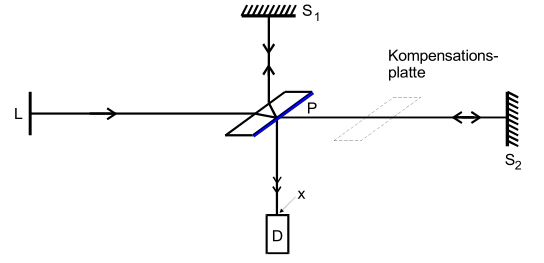
\includegraphics[width=\textwidth]{graphics/miif.JPG}
    \caption{Grundlegender Aufbau eines Michelson-Interferometers \cite{anleitung}}
    \label{fig:miif}
    \end{figure}
    \noindent
Dabei sorgt die semipermeable Platte P für die Strahlteilung. So geht ein Teil des von L emitierten Lichts durch P zu S2, während ein Strahl senkrecht auf S1 trifft. Um die beiden Strahlenbündel kohärent zu bekommen, muss ihr optischer Wegunterschied kleiner als die Kohärenzlänge von L sein. Man erreicht dies, indem man die Strecken zwischen S1 und P und S2 und P praktisch gleich lang wählt (bei exakter Gleichheit betrüge der Gangunterschied $\lambda/2$, sodass sich die Strahlenbündel auslöschen würden). Dazu wird in den Strahlweg zu S2 eine Kompensationsplatte gestellt, welche die gleiche Dicke und den gleichen Brechungsindex wie P besitzt, weil der Strahl zu S2 P nur einmal durchläuft, während der von S1 kommende Strahl dreimal durch P läuft bis er auf D trifft.
Nun werde ein Spiegel in Strahlrichtung um das Wegstück $\symup{\Delta} d$ verrückt. Mit der räumlichen Periode $\lambda/2$ gilt, mit $z$ als der Anzahl der dabei auftretenden Helligkeitsmaxima, für diese Anordnung:
\begin{equation}
    \label{eqn:Wlaenge}
    z \cdot \frac{\lambda}{2} = \Delta d
\end{equation}


\subsection{Messung des Brechungsindex n}
In \autoref{fig:brechindex} ist eine Apparatur zur Messung des Brechungsindex n mit einem Michelson-Interferometer dargestellt.
\begin{figure}[H]
    \centering
    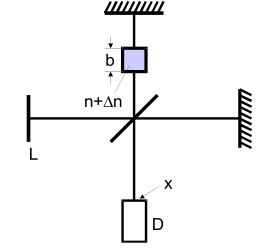
\includegraphics{graphics/brechindex.JPG}
    \caption{Apparatur zur Messung kleiner Brechungsindexunterschiede mit einem
    Michelson-Interferometer \cite{anleitung}}
    \label{fig:brechindex}
    \end{figure}
    \noindent
Mit dieser Messapparatur wird ein Strahlenbündel auf einem Wegstück der Länge b durch ein Medium mit dem Brechungsindex $n+\symup{\Delta} n$ geschickt. Der optische Wegunterschied zwischen den beiden Strahlenbündeln entspricht dann $b\symup{\Delta} n$.
Verändert man nun den Brechungsindex, indem man beispielsweise den Gasdruck in der Zelle verändert, werden am Detektor z Intensitätsmaxima detektiert. $z\lambda/2$ entspricht dann der optischen Weglängenänderung, also gilt: 
    \begin{equation}
        \label{eqn:brechungsindexa}
        b \cdot \symup{\Delta} n = z \frac{\lambda}{2}    
    \end{equation}
    \noindent
Die klassische Dispersionstheorie liefert als Zusammenhang zwischen dem Brechungsindex n und der Zahl N (N= die von der Lichtwelle zu erzwungenen Schwingungen pro Volumeneinheit angeregten Dipole) 
\begin{equation}
    n = \sqrt{1 + f(\lambda)N} \; .
\end{equation}
Für Gase im Bereich des sichtbaren Lichts kann dies zu 
\begin{equation}
    \label{eqn:nae}
    n = 1 + \frac{f}{2} N- ... 
\end{equation}
genähert werden. Außerdem wird die Gültigkeit der idealen Gasgleichung
\begin{equation}
    p V = R T 
\end{equation}
angenommen. Die Größe $N(p,T)$ ist proportional abhängig vom Druck $p$ und umgekehrt proportional abhängig von der Temperatur $T$, sodass die Zusammenhänge
\begin{align}
    \label{eqn:Ns}
    N(p,T) &= \frac{p}{T} \frac{T_0}{p_0} N_\text{L} & N(p',T) &= \frac{p'}{T} \frac{T_0}{p_0} N_\text{L}
\end{align}
gelten.
Dabei ist $p_0 = \SI{1013.2}{\milli\bar}$ der Normaldruck,
die Temperatur $T_0 = \SI{273.15}{\kelvin}$
und $N_\text{L}$ die Loschmidt'sche Zahl (Anzahl der Moleküle in 1 mol eines Gases).
Insgesamt erhält man dann aus \autoref{eqn:nae} und \autoref{eqn:Ns} für den Brechungsindex unter Normalbedingungen
    \begin{equation}
        \label{eqn:brechungsindex}
        n(p_0,T_0) = 1 + \symup{\Delta}n(p,p') \frac{T}{T_0} \frac{p_0}{p - p'} \; .
    \end{equation}
        